 
\subsubsection{Heterogeneous Single-ISA Processor Architectures}
Modern computing systems are constrained by \emph{dark silicon};
\emph{i.e.}, not all transistors can be powered at all times
\cite{DaSi2011,Venkatesh2010}.  The emergence of dark silicon has led
hardware architects to rethink processor design.  Recent designs
incorporate differing cores with a common instruction set and
programming model~\cite{Kumar.2005.heterogeneous,SulemanMQP09}.  Some
cores are complex with deep pipelines and large issue width, while
others are much simpler \cite{bigLittle}.  These \emph{heterogeneous
single-ISA} designs improve energy efficiency by executing computation
on the most appropriate type of core.

While these processors present a wide range of performance and energy
tradeoffs, they create a difficult scheduling problem.  Not only does
a software scheduler have to map tasks to core types, it also must
ensure that energy is minimized (to increase battery life) and that
critical power thresholds are not violated.  For example, the Exynos
5 processor (based on an ARM big.LITTLE architecture \cite{bigLittle})
has a 5.5W peak power that is nearly $2 \times$ the maximum
sustainable heat dissipation, limiting peak speed to less than 1
second \cite{exynos5}.  In addition, our prior work has shown that
this processor achieves greater energy efficiency as it slows down
\cite{Imes2014,Imes2014a}.  

Such a processor design creates both a challenge and an opportunity
for real-time embedded processing. The challenge is ensuring that
timing constraints are met while operating in the most
energy-efficient configuration.  The opportunity arises because the
processor is over-provisioned --- it has a much higher compute capacity
than it can safely sustain.  This extra compute capacity could be used
in short bursts to prevent timing errors.  The next section
illustrates these concepts with empirical results.

\subsubsection{Preliminary Results on Energy Efficiency and Timeliness
  for big.LITTLE Processors}

\begin{table*}[th]
\caption{Two embedded platforms with different configurable components.}
\label{tbl:machines}
\scriptsize 
\centering
\begin{tabular}{lcccccc}
  \textbf{Type} & 
  \textbf{Processor} &
  \textbf{Cores} & 
  \textbf{Core Types} &
  \textbf{Speeds (GHz)} &
  %\textbf{TurboBoost} &
  %\textbf{HyperThreads} & 
  \textbf{Idle Power (W)} & 
  \textbf{Configurations} \\
  \hline
  \hline
  Homogeneous   & Intel Haswell Mobile       & 2 & 1 & .6--1.5  & 2.5 & 45 \\
  big.LITTLE & Samsung Exynos5 Octa & 8 & 2 (A15, big \& A7, LITTLE) & .8--1.6 (A15) .5-1.2 (A7) & 0.12 & 69 \\
  \hline 
  \hline
\end{tabular}
\vskip -.7em
\end{table*}

We use an example application -- the x264 video encoder -- to compare
the different tradeoffs on an ARM big.LITTLE processor and a
traditional homogeneous multicore.  The video encoder is composed of
jobs, where each job encodes a frame. We instrument the encoder to
report job latency and measure each processor's energy consumption.
The two processors have different configurable resources, shown in
Table~\ref{tbl:machines}. The comparison of the two platforms is shown
in Table~\ref{tbl:machines}.

%\begin{comment}
\begin{figure}[h]
\vskip -1.8em
\subfloat[Energy/Latency Tradeoffs]{
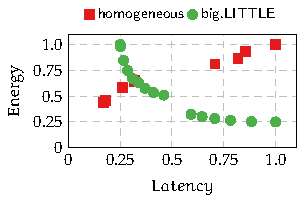
\includegraphics{pdf/rt-nsf-2016-figure0.pdf}
%\begin{tikzpicture}
\begin{centering}


\definecolor{s1}{RGB}{228, 26, 28}
\definecolor{s2}{RGB}{55, 126, 184}
\definecolor{s3}{RGB}{77, 175, 74}
\definecolor{s4}{RGB}{152, 78, 163}
\definecolor{s5}{RGB}{255, 127, 0}

% \begin{groupplot}[
%     group style={
%         group name=plots-labeltop,
%         group size=2 by 1,
%         xlabels at=edge top,
%         xticklabels at=edge top,
%         vertical sep=5pt,
%     },
% xlabel near ticks,
% height=4cm,
% width=0.5\textwidth,
% xtick=\empty,
% ytick=\empty,
% xmin=0,
% xmax=20,
% ymin=0,
% ymax=1.5,
% ]
% \nextgroupplot[xlabel={\footnotesize $\mathsf{Performance}$ (normalized latency)}]
% \nextgroupplot[xlabel={\footnotesize $\mathsf{Power}$ (Watts)}]
% %\nextgroupplot[xlabel={\footnotesize $\mathsf{Accuracy}$}]
% %\nextgroupplot[]
% %\nextgroupplot[]
% %\nextgroupplot[]
% \end{groupplot}

\begin{groupplot}[
    group style={
        group name=plots,
        group size=1 by 1,
        xlabels at=edge bottom,
        xticklabels at=edge bottom,
        vertical sep=5pt
    },
xlabel={\footnotesize $Latency$ 
%(normalized to worst case)
},
xlabel near ticks,
height=3.5cm,
%width=0.5\textwidth,
width = 4.2cm,
xmajorgrids,
ymajorgrids,
grid style={dashed},
xtick={0,0.25,0.5,0.75,1.0},
xticklabels={0,0.25,0.5,0.75,1.0},
xticklabel style={font=\footnotesize},
xmin=0,
xmax=1.1,
yticklabel pos=left,
enlargelimits=false,
tick align = outside,
tick style={white},
xticklabel shift={-5pt},
yticklabel shift={-5pt},
ylabel shift={-2pt},
ylabel style={align=center},
unbounded coords=jump,
]

\nextgroupplot[ylabel={\footnotesize Energy}, 
%ylabel shift={6mm},
ytick={0,0.25,0.5,0.75,1.0},
yticklabels={0,0.25,0.5,0.75,1.0},
yticklabel style={font=\footnotesize},
ymin=0,
ymax=1.1,
legend entries={{\scriptsize $\mathsf{Vaio}$},{\scriptsize $\mathsf{ODROID}$}},
legend style={draw=none,at={(0.5,1.35)},anchor=north,legend columns=4,line width=5pt},
]
\addplot[thick, solid, color=s1, only marks, mark=square*] table[x index=2,y index=5,col sep=tab] {img/vaio-tradeoffs.txt};
\addplot[thick, solid, color=s3, only marks, mark=*] table[x index=2,y index=5,col sep=tab] {img/odroid-tradeoffs.txt};


\end{groupplot}
\end{centering}

\end{tikzpicture}

\label{fig:x264-motivation-tradeoffs}}
\subfloat[Heuristic Energy Consumption]{
%\begin{tikzpicture}

\begin{groupplot}[
    group style={
        group name=plots,
        group size=1 by 1,
        xlabels at=edge top,
        xticklabels at=edge top,
        vertical sep=5pt
    },
axis x line* = top,
xlabel near ticks,
major x tick style = transparent,
height=3.5cm,
%width=0.95\columnwidth,
width=4.2cm,
xmin=0,
xmax=3,
enlargelimits=false,
tick align = outside,
tick style={white},
ytick=\empty,
xtick=\empty,
xticklabels={},
yticklabels={},
]
\nextgroupplot[ylabel={\footnotesize Energy},
ylabel shift={6mm},
ymin=0,
ymax=1,
]


\end{groupplot}

\begin{groupplot}[
    group style={
        group name=plots,
        group size=1 by 1,
        xlabels at=edge bottom,
        xticklabels at=edge bottom,
        vertical sep=5pt
    },
axis x line* = bottom,
xlabel near ticks,
major x tick style = transparent,
height=3.5cm,
%width=0.95\columnwidth,
width=4.2cm,
xmin=0,
xmax=3,
enlargelimits=false,
tick align = outside,
tick style={white},
ytick=\empty,
xticklabel shift={-5pt},
%x tick label style={rotate=0, anchor=south},
xlabel={\footnotesize $Platform$},xtick={1,2,3},
xticklabels={{\scriptsize $\mathsf{Vaio}$},
{\footnotesize $\mathsf{ODROID}$}},
ymin=1,
ymax=2.25,
ytick={1.0,1.25,1.5,1.75,2.0},
yticklabels={1.00,1.25,1.50,1.75,2.00,2.25},
legend cell align=left, 
legend style={ column sep=1ex },
ymajorgrids,
grid style={dashed},
]
\nextgroupplot[ybar=\pgflinewidth,
bar width=5pt,
legend entries = {{\scriptsize $\mathsf{never~idle}$},{\scriptsize $\mathsf{race~to~idle}$}},
legend style={draw=none,legend columns=2,at={(0.5,1.35)},anchor=north},
]
\addplot table[x index=0,y index=2, col sep=space] {img/heuristics2.txt};
\addplot table[x index=0,y index=3, col sep=space] {img/heuristics2.txt};


\end{groupplot}

\end{tikzpicture}

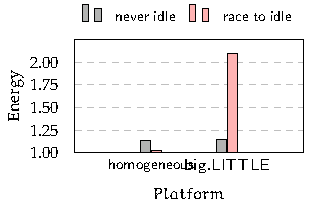
\includegraphics{pdf/rt-nsf-2016-figure1.pdf}
\label{fig:x264-motivation-heuristics}}
%  \subfloat[Intel Haswell]%
%  {\input{img/tradeoffs-v.tex}%
%  \label{fig:pwr-perf-vaio}}
\subfloat[ARM big.LITTLE Power/performance]%
{
%\begin{tikzpicture}
\begin{centering}


\definecolor{s1}{RGB}{228, 26, 28}
\definecolor{s2}{RGB}{55, 126, 184}
\definecolor{s3}{RGB}{77, 175, 74}
\definecolor{s4}{RGB}{152, 78, 163}
\definecolor{s5}{RGB}{255, 127, 0}

\begin{groupplot}[
    group style={
        group name=plots,
        group size=1 by 1,
        xlabels at=edge bottom,
        xticklabels at=edge bottom,
        vertical sep=5pt
    },
xlabel={\footnotesize $Power$ 
%(normalized to worst case)
},
xlabel near ticks,
height=3.5cm,
width=0.3\columnwidth,
%width = 4.5cm,
xmajorgrids,
ymajorgrids,
grid style={dashed},
xtick={0,0.25,0.5,0.75,1.0},
xticklabels={0,0.25,0.5,0.75,1.0},
xticklabel style={font=\footnotesize},
xmin=0,
xmax=1.1,
yticklabel pos=left,
enlargelimits=false,
tick align = outside,
tick style={white},
xticklabel shift={-5pt},
yticklabel shift={-5pt},
ylabel shift={-2pt},
ylabel style={align=center},
unbounded coords=jump,
]

\nextgroupplot[ylabel={\footnotesize Performance}, 
%ylabel shift={6mm},
ytick={0,0.25,0.5,0.75,1.0},
yticklabels={0,0.25,0.5,0.75,1.0},
yticklabel style={font=\footnotesize},
ymin=0,
ymax=1.1,
legend entries={{\scriptsize $\mathsf{1}$},{\scriptsize $\mathsf{2}$},{\scriptsize $\mathsf{3}$},{\scriptsize $\mathsf{4}~cores$},{\scriptsize $\mathsf{sustainable~power}$}},
legend style={draw=none,at={(0.5,1.35)},anchor=north,legend columns=5,line width=5pt},
]
\addplot[thick, solid, color=s4, only marks, mark=square*] table[x index=15,y index=14,col sep=comma] {img/tradeoffs-o.csv};
\addplot[thick, solid, color=s3, only marks, mark=square*] table[x index=13,y index=12,col sep=comma] {img/tradeoffs-o.csv};
\addplot[thick, solid, color=s2, only marks, mark=square*] table[x index=11,y index=10,col sep=comma] {img/tradeoffs-o.csv};
\addplot[thick, solid, color=s1, only marks, mark=square*] table[x index=9,y index=8,col sep=comma] {img/tradeoffs-o.csv};
\addplot[very thick, dashed, black] coordinates {(.49,0) (.49, 1)};


\end{groupplot}
\end{centering}

\end{tikzpicture}
%
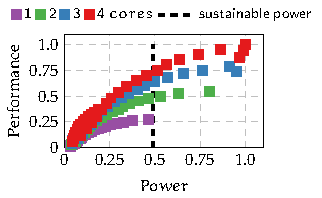
\includegraphics{pdf/rt-nsf-2016-figure2.pdf}
\label{fig:pwr-perf-odroid}}
\caption{Characterization of ARM big.LITTLE processor for latency and
  energy tradeoffs (a), different resource allocation heuristics (b),
  and power and performance tradeoffs (c).}
\label{fig:x264-motivation}
\end{figure}
%\end{comment}

Figure~\ref{fig:x264-motivation} shows the latency and energy
tradeoffs of the video encoder on our two test platforms.  The
different shapes of these tradeoff spaces on the ARM big.LITTLE and
the homogeneous system lead to different optimal resource allocation
strategies. Empirical studies show that the \emph{race~to~idle}
heuristic, which makes all resources available and then idles after
completing a job, is near optimal on systems like the homogeneous
processor~\cite{PowerSlope,Hoelzle2009,google2,Imes2014,HotPower}.  On
systems like the big.LITTLE processor, recent approaches save energy
by keeping the system constantly busy and
\emph{never~idle}~\cite{Carroll13,LeSueur11,Imes2014,HotPower}.

To demonstrate how different scheduling decisions affect the different
platforms, we compare the energy consumption of both race-to-idle and
never-idle.  We set a latency target equal to the worst observed
latency for this application on each processor and measure the energy
consumption of encoding 500 video frames using each heuristic.
Figure~\ref{fig:x264-motivation} shows the results, normalized to
the optimal energy found by measuring every possible resource
configuration for each frame.  Both heuristics meet the latency
target, but their energy consumptions vary tremendously. On the
homogeneous processor, \emph{race~to~idle} is near optimal, but
\emph{never~idle} consumes 13\% more energy.  Conversely,
\emph{never~idle} is near optimal for the heterogeneous processor, but
\emph{race~to~idle} consumes $2 \times$ more energy.

Finally, we note that due to the presence of dark silicon in the ARM
big.LITTLE, there is additional compute power that can be brought to
bear temporarily, but cannot be sustained.
Figure~\ref{fig:x264-motivation} illustrates this property as it
shows the power and performance tradeoffs for the video encoder (all
normalized so that 1 is the maximum).  The horizontal dashed line
represents the maximum sustainable power without active cooling.  Note
two important properties of this figure: 1) the maximum performance is
almost 33\% higher than the sustainable performance and 2) the only
configurations that are guaranteed never to violate safe operating
power dissipation are those that use the little cores.

On the whole, the results in Figure~\ref{fig:x264-motivation} demonstrate
two key points that will guide our proposed research:
\begin{itemize}
\item The conventional approach of allocating all resources and
transitioning to a low power idle state is extremely inefficient on
the big.LITTLE processor.  
\item The big.LITTLE processor can reach speeds of up to $1.33 \times$
  faster than it can safely sustain.
\end{itemize}
